\section{Use case maps för implementationsarkitektur}
\label{sec:use_case_implementation}

\begin{figure}[h]
    \centering
    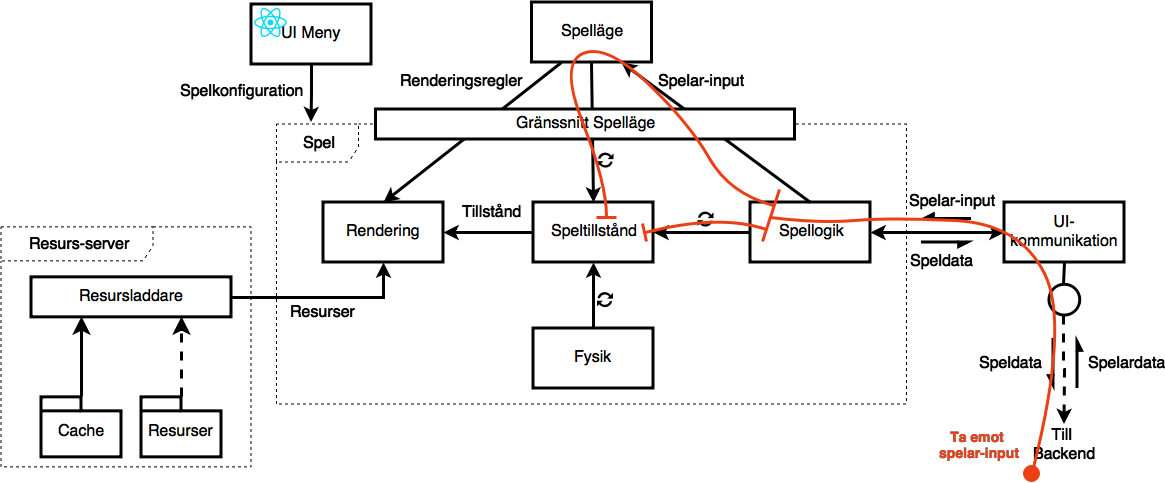
\includegraphics[scale=0.4]{implementation_use_case_ta_input}
    \caption{Use case map för att ta emot spelar-input}
    \label{fig:use_case_implementation_input}
\end{figure}

\begin{figure}[h]
    \centering
    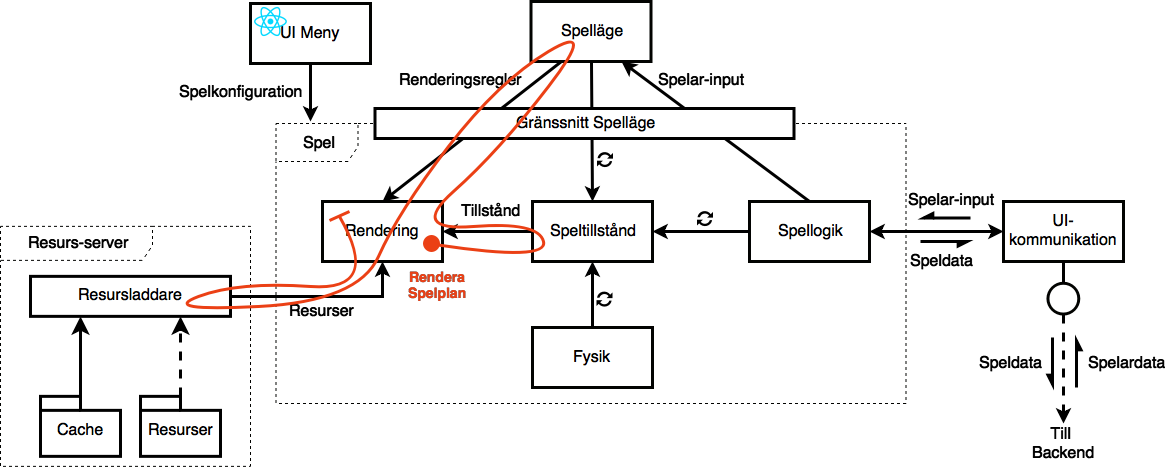
\includegraphics[scale=0.4]{implementation_use_case_rendera_spelplan}
    \caption{Use case map för att rendera spelplanen}
    \label{fig:use_case_implementation_rendera}
\end{figure}

\pagebreak

\section{Impact maps för implementationsarkitektur}
\label{sec:impact_implementation}

\begin{figure}[h]
    \centering
    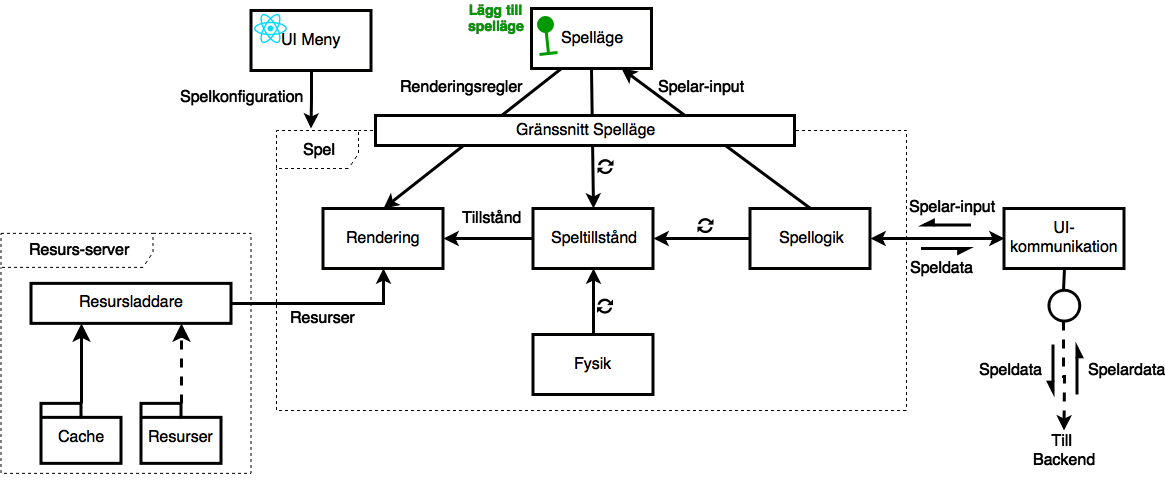
\includegraphics[scale=0.4]{implementation_impact_nytt_spellage}
    \caption{Impact map för att lägga till ett nytt spelläge}
    \label{fig:impact_implementation_spellage}
\end{figure}

\begin{figure}[h]
    \centering
    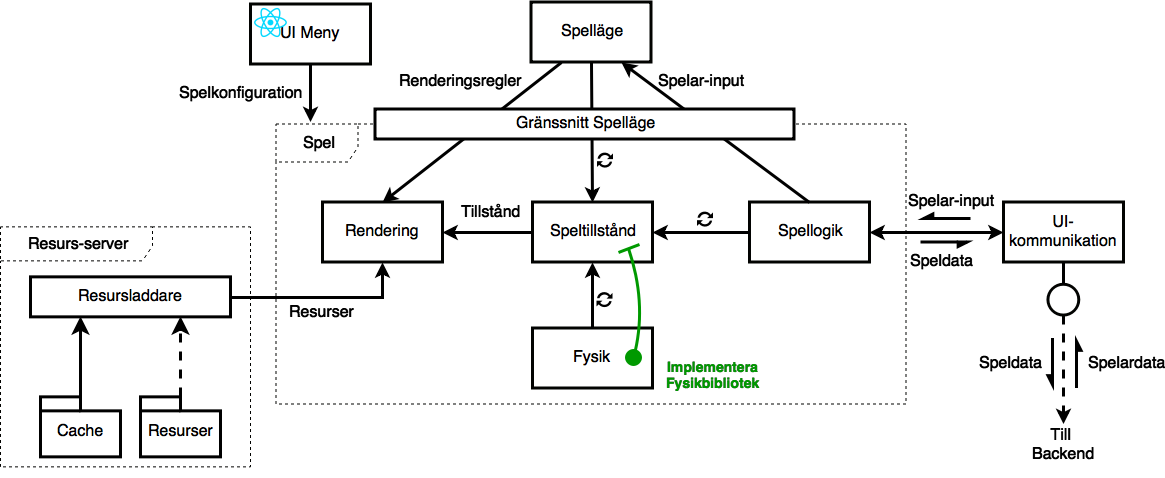
\includegraphics[scale=0.4]{implementation_impact_fysikbibliotek}
    \caption{Impact map för att implementera ett färdigt fysikbibliotek}
    \label{fig:impact_implementation_fysikbibliotek}
\end{figure}

\begin{figure}[h]
    \centering
    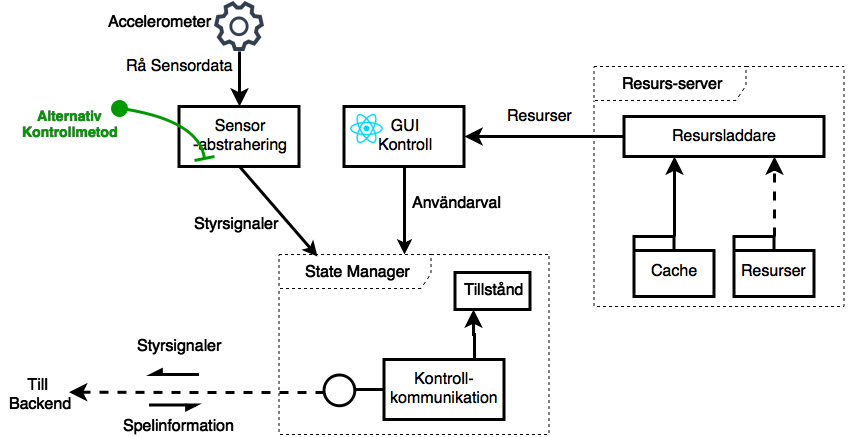
\includegraphics[scale=0.4]{implementation_impact_alternativ_kontroll}
    \caption{Impact map för att lägga till en alternativ kontrollmetod}
    \label{fig:impact_implementation_alt_kontroll}
\end{figure}
